% Primarily this section should be about scientific methods and theories you need to evaluate/compare/invent to solve your problems from 1.3.
% In some cases it may be ok to describe different technologies, but the purpose is to describe something and then draw a conclusion from that.
% Example, if you decide to discuss different databases, it may be for the purpose of selecting the best type for your implementation later on (based on for example data representation, scalability, speed, etc.).
% Optimally the problems in 1.3 are not solved by anyone else yet, in which case this section needs to describe how to solve them (new algorithms, mathematical approaches, etc.).
 
% This section can have a lot of subsections (3.1, 3.2, 3.3, etc).


% TODO: Explain DWARF Sections
The \gls{DWARF} format is divided into sections that all contain unique information with some few small exceptions.
These sections use offsets from the start of other sections to point to information in the other section, most of these offsets can be found in specific \gls{DWARF} attributes.
The figure \ref{fig:dwarfsections} shows all the \gls{DWARF} sections and which ones point to each other.


%All of the sections are not in every version of \gls{DWARF} and are sometimes changed from version to version.
%Thus the following explanations are specific for \gls{DWARF} version $4$ but can sometimes also apply for other versions, checkout Appendix F in \cite{dwarf} for more information on the changes done from older versions.


\begin{figure}[h]
	\centering
	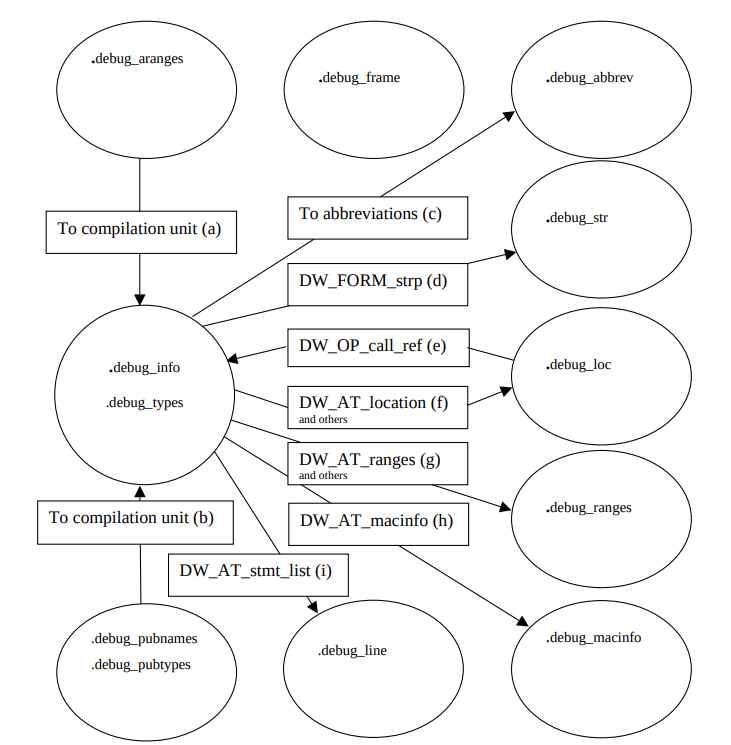
\includegraphics[width=0.9\textwidth]{dwarf-sections.png}
	\caption{Diagram of all the different \gls{DWARF} sections and their relations to each other.}
	\label{fig:dwarfsections}
\end{figure}


\subsubsubsection{\emph{.debug\_abbrev}}
The \gls{DWARF} section \emph{.debug\_abbrev} contain all of the abbreviation tables which are used to translate abbreviation codes into its official \gls{DWARF} names.
Some of the things these abbreviation code are used for are \gls{die} tags and \gls{die} attribute names.
To translate a abbreviation code one has to compare each entry until the one with the matching abbreviation code is found.
Checkout section $7.5.3$ in \cite{dwarf} to learn more.


\subsubsubsection{\emph{.debug\_aranges}}
The \gls{DWARF} section \emph{\.debug\_aranges} is used to lookup compilation units using machine code addresses.
Each compilation unit has a range of machine code addresses that are the addresses that the compilation unit have information on.
These ranges consists of a start address followed by a length.
Thus to find the compilation unit having the information about the current state.
The user only needs to check if the current address is between the start address and the start address plus the length.
To read more about this section checkout section $6.1.2$ in \cite{dwarf}.


\subsubsubsection{\emph{.debug\_frame}}
In the \gls{DWARF} section \emph{.debug\_frame} the information needed to virtually unwind the call stack is kept.
This section is completely self-contained and is made up of two structures called \acrfull{cie} and \acrfull{fde}.
Virtually unwinding the call stack is complex, thus to learn more about that checkout section \ref{sec:stacktrace} and  section $6.4.1$ in \cite{dwarf}


\subsubsubsection{\emph{.debug\_info}}
Most of the information about the source code is stored in \glspl{die} which are low-level representation of the source code.
\glspl{die} have a tag that describes what it represents, an example tag is \emph{DW\_TAG\_variable} which means that the \gls{die} represents a variable from the source code.
All \glspl{die} are stored in trees, which is a common data structure.
Each compilation unit will have at least on of these trees made up of \glspl{die} and each tree is stored in a \gls{DWARF} unit.
The trees are structured the same as the source code, which makes it easy to relate the source code to the machine code.

The section \emph{.debug\_info} consist of a number of these \gls{DWARF} units and some other debug information.
This is one of the most important sections in \gls{DWARF} because it is used to relate the state of the debug target and the source code, and vice versa.


\subsubsubsection{\emph{.debug\_line}}
The \gls{DWARF} section \emph{.debug\_line} holds the needed information to find the machine addresses which is generated from a certain line and column in the source file.
It is also used to store the source directory, file name, line number and column.
Then the \glspl{die} will store pointers to the source location information in the section \emph{.debug\_line} enabling the debugger to know the source location of a \gls{die}.
The section $6.2$ in \cite{dwarf} explains in more detail how this information is stored in the \emph{.debug\_line} section.


\subsubsubsection{\emph{.debug\_loc}}
The location of the variables values are stored in location lists, each entry in the list holds a number of operation that can be used to calculate the location of the value.
All of the location lists are stored in the section \emph{.debug\_loc} and are pointed to by \glspl{die} in the \emph{.debug\_info} section.
These offsets are most commonly found in the attribute \emph{DW\_AT\_location} which is often present in \glspl{die} representing variables.
The relation between these two sections can be seen in the figure \ref{fig:dwarfsections}.


\subsubsubsection{\emph{.debug\_macinfo}}
In the section \emph{.debug\_macinfo} the macro information is stored.
It is stored in entries that each represents the macro after it has been expanded by the compiler.
These entries are also pointer to by \glspl{die} in the \emph{.debug\_info} section and those pointers can be found in the attribute \emph{DW\_AT\_macinfo}.
This section is a little bit complex thus to learn more about it read section $6.3$ in \cite{dwarf}.


\subsubsubsection{\emph{.debug\_pubnames} and \emph{.debug\_pubtypes}}
There are two sections for looking up compilation units by the name of functions, variables, types and more.
The first one is \emph{.debug\_pubnames} which is for finding functions, variables and objects and the other one is for finding types, this section is called \emph{.debug\_pubtypes}.
Both of these are meant to be used for fast lookup of what unit the search information is located in.
Checkout section $6.1.1$ in \cite{dwarf} for more information.


\subsubsubsection{\emph{.debug\_ranges}}
\Glspl{die} that have a set of addresses that are non-contiguous will have an offset to the section \emph{.debug\_ranges} instead of having a address range.
The offset points to the start of a range list that contain range entries which are used to know which of the machine code addresses the \gls{die} is active.
The \gls{DWARF} section \emph{.debug\_ranges} is used for storing these lists of ranges.
Check out section $2.17$ in \cite{dwarf} to learn more about code addresses and ranges.


\subsubsubsection{\emph{.debug\_str}}
The \gls{DWARF} section \emph{.debug\_str} is used for storing all the strings that is in the debug information.
An example of these strings are the names of the functions and variables.
These string are found using a offset that are located in the attribute \emph{DW\_AT\_name}.
The attribute is found in the function and variable \glspl{die} and the offset is in the form of \emph{DW\_FROM\_strp}.


\subsubsubsection{\emph{.debug\_type}}
The \gls{DWARF} section \emph{.debug\_type} is similar to section \emph{.debug\_info} in that it is also made up of units with each a tree of \glspl{die}.
The difference is that the \glspl{die} are a low-level representation of the types in the source code.

